\documentclass[11pt]{article}
\usepackage{geometry} % see geometry.pdf on how to lay out the page. There's lots.
\usepackage{hyperref}
\usepackage{graphicx}
\usepackage{gensymb}
\usepackage[affil-it]{authblk}
\usepackage[toc,page]{appendix}
\usepackage{pifont}
\usepackage{amsmath}
\usepackage{amssymb}
\usepackage{relsize}
\usepackage{draftwatermark}
\usepackage[mathscr]{eucal}
\usepackage{amsmath, amssymb, graphics, setspace}
\usepackage[english]{babel}
 
\newcommand{\mathsym}[1]{{}}
\newcommand{\unicode}[1]{{}}

\newtheorem{exercise}{Exercise}
\newtheorem{problem}{Problem}

\SetWatermarkText{DRAFT}
\SetWatermarkScale{6}
\SetWatermarkLightness{0.95}

\DeclareMathOperator{\atantwo}{atan2}
\DeclareMathOperator{\sign}{sign}
\DeclareMathOperator{\sense}{sense}

% \geometry{letter} % or letter or a5paper or ... etc
% \geometry{landscape} % rotated page geometry

% See the ``Article customise'' template for come common customisations

\title{Open Recreational Problems: Simplex Chains}
\author{Robert L. Read
  \thanks{read.robert@gmail.com}
}
\affil{Founder, Public Invention, an educational non-profit.}


\date{\today}

%%% BEGIN DOCUMENT
\begin{document}

\maketitle

%% \tableofcontents

\section{License}
This work is Copyright 2018, Robert L. Read, but licensed under the Creative Commons Attribution-ShareAlike 4.0 (CC BY-SA 4.0).
\url{https://creativecommons.org/licenses/by-sa/4.0/}. This means you are free to share and adapt this work work, giving appropriate credit
and maintaining the same license.

Contributions and suggestions from the reader are encouraged!

\section{Introduction}

{\em
Note: This is a work in progress as a preparation for the Public Invention Mathathon planned for Nov. 30th-Dec. 2nd 2018.
Please read it as work designed to give a flavor of the problem area rather than a technical paper being prepared for publication.
}

The term {\em simplex} means the simplest regular polyhedron. In two dimensions, a simplex is an equilateral triangle.
In three dimensions, a simplex is a regular tetrahedron.

Define a {\em simplex chain} to be a figure of many simplices adjoined face-to-face by a particular rule.
The dimensionality of a face is always one less than the dimensionality of the space. In two dimensions,
a simplex chain is a series of adjoined equilateral triangles joined edge-to-edge.

Let us number the simplices in a chain starting from $0$. Then we can define a simplex chain via a rule
that says which edge of the $n$th simplex to attach the $n+1$th simplex to. In two dimensions, we can
label the edge of the last triangle in simplex chain as {\em anti-clockwise} or {\em clockwise}, or just
{\em left} and {\em right}.

If is clear that the rules ``always go left'' ``always go right'' produced a pretty hexagon, but then starts putting the triangles
right where one already is.

The rule ``go left if $n$ is even, right if it is odd'' is a bit more interesting; it produces a ``ladder'' that goes off
in a straight line. That is, the whole figure is contained with in two parallel lines separated by the height of the triangle.

\begin{figure}
     \centering
     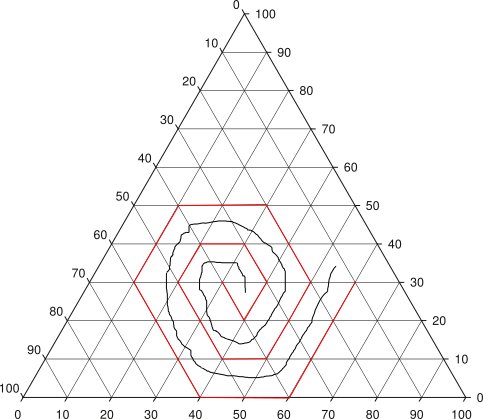
\includegraphics[width=0.65\textwidth]{figures/2DSpaceFilling.png}
     \caption{A Space Filling Spiral}
  \label{fig:equitetrabeam}
\end{figure}




With the help of David Jeschke, we have written a website\url{https://pubinv.github.io/Mathathon-2018-Simplex-Chains/platforms/index.html}
designed to allow graphic and interactive play of these concepts.  Specifically it should assist in solving this exercise:

\begin{problem}
  There is probably a simplex chain rule which tiles the entire plane with equilateral triangles. Can you define it?
\end{problem}

This website will likely evolve faster than this document!

\subsection{The nature of this work}

The problems posed here to make the Public Invention Mathathon interesting exist at the intersection of mathematics and
computer science. The work is motivated by mechanical engineering and robotics. In particular, there is an entire class
of robots, called the {\em tetrobot}, built entirely out of simplices which can change their member lengths. A few
dozen academic papers have been published on this subject in the last 25 years.

\subsection{The mechanically interesting shapes}

Although simplex chains are interesting in their own right purely theoretically and for recreation,
they are of practical applied value as well.
Mechanical and structural engineers are interested in simplex chains because when constructed out of real, physical
members in the shape of the simplex chain, they may form rigid and structural strong shapes.
For example, many trusses, used to hold up bridges and the roofs of buildings, are in fact simplex chains.

In two dimensions, there are a number of shapes which are interesting not just to mathematicians, but
to engineers and architects. Often, these shapes are made of {\em trusses} which approximate
geometric forms.
In two dimensions the mechanically interesting shapes are:
\begin{itemize}
\item The line
\item The triangle
\item The circle
\item The spiral
\item The sine wave
\end{itemize}

The line is used to make columns and beams. The triangle is the basis of all trusses.
Fractions of circles are arcs used to make bridges. Spirals are used to make clock springs.
The sine wave is similar to the barrel vault and is used to make corrugated roofs and cardboard
and baffles.
Note that the triangle and the circle are closed shapes, the others are not.

General structures in three dimensions made by structural and mechanical engineers are
called {\em space frames}. However, many space frames also follow geometric patterns.
In three dimensions the mechanically interesting shapes are:
\begin{itemize}
\item The beam
\item The triangle
\item The tetrahedron
\item The ring
\item The helix
\item The spiral
\end{itemize}

The beam, the triangle, the ring and the spiral can exist in a narrow space, like inside a wall,
so they are similar to their 2-d analogs, and used for the same purposes.

The helix is used to make staircases and springs and heat exchangers.

Note that the ring and the triangle are a closed shape, the others are not.
The helix does not really exist in two space, although the others do.

The only four-dimensional shape I can conceptualize is that of the
beam: that is, a region close to a line embedded in 4-space.

\section{On ``Open Problems''}

This mathathon is focused on real {\em unsolved open problems.}
Usually when we say ``open problem'' in mathematics we mean ``unsolved, probably has a clear objective solution, is valuable,
and is not obvious.''
Open problems you hear about are mostly ones that have been studied a lot and remain unsolved, and are therefore probably difficult problems.
However, in this mathathon, many of the open problems are probably easy---they are open and unsolved because nobody has yet
cared to look very closely at them.  However, they are still valuable. Hopefully the problems in this research-a-thon are ``real'', even if they
not as ``hard'' as those professional researchers talk about.

We will give opinions about problems on a scale\footnote{This scale is inspired by Prof. Norman J Wildberger, who has ranked famous open problem using a similar
  (but much more difficult!) gamut.} of $1-10$, with $1$ being quite easy and $10$ being very difficult. Problems of difficulty $1,2,3$
are generally ``easy'', those of ``8,9,10'' hard.  A problem of difficulty $10$ is assumed to be publishable in a not-very-prestigious forum, though
possibly easier problems will also be of interest. 

\section{Some Easy Problems on Generators of Regular 2D Simplex Chains}

\subsection{Generators}

Define a {\em regular simplex chain generator} to be a function takes natural numbers and returns a symbol from the set $\mathbb{N} \mapsto \{L,R,S\}$,
  for {\em left}, {\em right}, and {\em stop}. The generator generates a simplex chain by defining to which edge a new triangle should
  be attached. That is, measured from the direction of a previous edge, should $n$th addition of a triangle be made by adding it
  to the left or right edge?

  Here is an example of a generator in JavaScript:
\begin{verbatim}
function hex_generator(n) {
    return ((n < 6) ? "L" : "S");
}
\end{verbatim}
It produces a simple hexagon. We will assume that regular triangles have unit side length.

Although a 2D simplex chain exists in $\mathbb{R}^2$, a generator is a much simpler object.  It is somewhat easier to ask questions about
generators.

\begin{problem}[GEN-BEAM]
  (Easy 1) Can you create a generator which creates a beam?
\end{problem}
\begin{problem}[GEN-PLANE]
(Easy 2) Can you create a generator which fills the plane?  
\end{problem}
\begin{problem}[GEN-CIRCLE]
  (Easy 3) Can you create a generator which completely covers a circle or radius $r$ with no unnecessary triangles?
\end{problem}
\begin{problem}[GEN-SPIRAL]
  (Medium 4) Can you create a generator which creates golden spiral?
\end{problem}
\begin{problem}[GEN-SINWAVE]
  (Medium 4) Can you create a generator which completely and minimal covers a sinusoidal wave?
\end{problem}
\begin{problem}[GEN-LOGSPIRAL]
  \label{probgenlogspiral}
  (Medium 5) Can you create a generator which defines a logarithmic spiral which does not rely on mapping first to the Cartesian plane?
  (variations are other forms of spirals.)
\end{problem}
Problem \ref{probgenlogspiral} raises an interesting issue. It is of course possible to create an algorithm which solves a problem in Cartesian space, and then
map this back to the turnings of the generator. However, it would be more elegant to create an algorithm which never in fact uses real numbers.


\begin{problem}[GEN-ARBITRARY]
(Medium 4 R2D-10) What is the best way to define ``approximating'' an arbitrary  curve with a simplex chain? Is it the sum of the distances of the centroid to the curve?
  Or some notion based on completely covering the curve and not self-colliding?  
\end{problem}

Finally, here is a problem of some practical value to mechanical engineers:
\begin{problem}[GEN-BRESENHAM]
  (Medium 6) Can you create a generator draws a figure from the origin to any particular triangle as smoothly as possible as contained
  between the closest parallel lines as possible? (This is analogous to Bresenham's \url{https://en.wikipedia.org/wiki/Bresenham%27s_line_algorithm}
    line drawing algorithm with connected triangles pixels.)
\end{problem}

\begin{problem}[GEN-PERIODICITY]
(Hard 7 R2D-08) Can we define a notional of ``translational periodicity'' of a regular simplex chain? That is, can we prove that
  a given rule for producing a simplex chain produces of series of translations of a smaller simplex chain? For example,
  if we have a simplex chain which approximates a sine wave or sawtooth wave, can prove that with a periodicity of $k$ it
  is self-similar?  
\end{problem}

\subsection{Two dimensions}

\subsection{Numbering of the Regular Triangle Space}

Any Regular 2D Simplex Chain, although it may be thought of as points in $\mathbb{R}^2$, may also be thought of as simply
selecting a set of triangles in an abstract space, which we call the {\em Triangle Space}, which is $\mathbb{Z}^2$. By convention,
we begin numbering the Triangle Space at a equilateral triangle point upward, whose apex is at the origin.  Then any triangle can be
named by $(x,y)$, where $y=0$ on is the horizontal row of triangles below the $x$-axis. A triangle at position $x$ has an apex
pointing either upward or downward at position $x/2$.

\begin{figure}
     \centering
     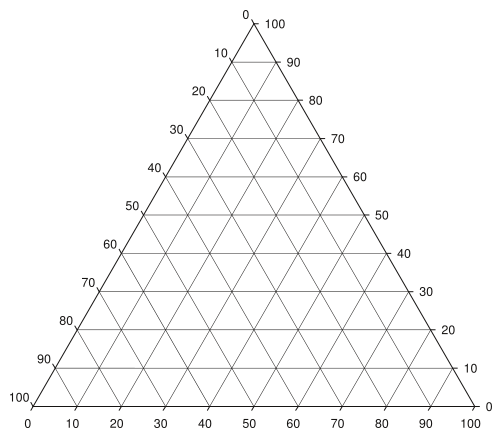
\includegraphics[width=0.65\textwidth]{figures/Triangle_Plot_-_Major_grid_lines.png}
     \caption{Triangle Space Numbering}
  \label{fig:equitetrabeam}
\end{figure}

\footnote{ Amit proposes a different numbering scheme for regular triangles:
  \url{http://www-cs-students.stanford.edu/~amitp/game-programming/grids/})
}

\subsection{On the reachability of points}

Although too simple for a professional mathematician in two dimensions, let us consider the problem of {\em reaching} certain regions
or points with a simplex chain from a starting point.

Let us for the time being consider {\em regular} simplex chains.  In the Cartesian plane, it is pretty clear that any point can {\em reached},
that is, intersected, by a simplex chain of finite length. Developing an algorithm to produce such a chain from the coordinates of a point
is an easy problem. We could then pose questions about the shortest such chain, or the number of such chains.

Now consider the problem of reaching a point in 3D with a simplex chain formed only of regular tetrahedra.
\begin{problem}[REGULAR REACHABILITY]
  (Hard 9)  Given a a point in 3-space, produce a regular simplex chain of tetrahedra starting at the origin.
  Give the shortest simplex chain which intersects the point.
\end{problem}
This is a much harder problem.

It seems likely that any point can be intersected, except perhaps points very close to the starting point. Producing an algorithm to do so
is more of a challenge. This is a very interesting problem to mechanical engineers, robotocists, and possibly molecular scientists.

Now if instead of merely {\em intersecting} a point with the body of simplex we instead seek to move the {\em apex} of a tetrahedra close
to the point, we have a real challenge.
\begin{problem}
  (Hard 9) Given a point in 3-space and a distance $d$, produce a shortest regular simplex chain starting at the origin whose apex
  is within $d$ of the point.
\end{problem}

\begin{problem}
(Hard 9) Can we come arbitrarily close to a point with arbitrary length chains?
\end{problem}

\subsection{A diversion}
An interesting, if somewhat wild idea, is to build a coordinate system around points based on reaching them with simplex chains. In this model
we do not start with the Cartesian plane; rather we ``name'' points by the simplex chain we reaches them. What is the nature of a space
of such points? 



\section{Relaxations of Regularity}
\subsection{Boundedness}

If we relax the rule that all the lengths of simplex are exactly the same, then it becomes possible to create new figures which are
very close to regular. In particular we can define a simplex chain, or any structure, be {\em $x$-bounded} if the ratio of the longest edge
in the figure to the shortest edge is $x$.

We can then ask questions (in 3D) such as:

\begin{problem}[SMALLEST-TORUS]
(Hard 9)  What is the smallest number of tetrahedra needed to define an $b+c/b$ torus as a function of $b$ and $c$?
  \end{problem}

Or:

\begin{problem}[TORUS-BOUNDEDNESS]
(Hard 9)  What is the lowest $x$-boundedness of a figure that defines a torus?
  \end{problem}

A bound on this number can be given based on my previous work; however, there is almost certainly a better solution that ``twists'' about the torus.

One way to investigate this is simply to place points on the surface of a torus and draw edges between them so as to create an irregular tetrahelix.

\subsection{Rational Regularity}

Define a {\em $k$-regular tetrahelix} to be tetrahelix have at most $k$ distinct edge lengths.
Define a {\em $k$-regular rational tetrahelix} to be a $k$-regular tetrahelix in which all lengths are rational.

We can then ask:

\begin{problem}[SMALLEST-HAS-HOLE]
  What is the smallest closed $k$-regular/$k$-regular rational tetrahelix with a hole in each of these dimensions?
\end{problem}

Note: There exists a 3-regular rational tetrahelix that is a straight line, or a beam.


\section{Three dimensions}

The problem of simplex chains in three dimensions is much more interesting. In particular, there is a structure known as the
tetrahelix which is analogous to a 2D ladder: it fits inside a cylinder. That is, it is a ``straight'', uncurved stack
of tetrahedra extending infinitely.


\begin{figure}
  \centering
     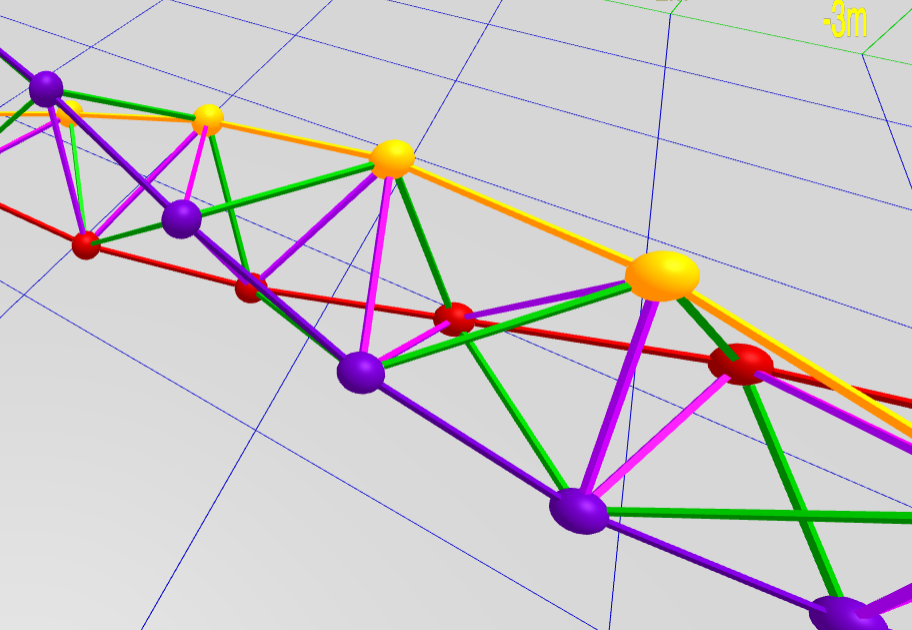
\includegraphics[width=0.45\textwidth]{figures/BCHelixCloseUp.png}
     \caption{BC Helix Close-up (partly along axis)}
  \label{fig:closeup}     
\end{figure}



In order to produce a tetrahelix as a simplex chain, we must have a labeling scheme for the faces of a tetrahedron.
Although symmetric, the first tetrahedron has 4 faces against which we can place the second tetrahelix.
Having placed the second tetrahelix, there are 3 faces against which we can place the third, if we
seek not to collide with the first. These 3 are symmetric; there is no good way to distinguish them,
so in a sense it doesn't matter where we place the third.

But when we come to place the fourth, the figure changes. The three tetrahelices have a clear ``spine''. If we
place the fourth on the face that does not touch the spine, we start to create a shape somewhat like a spindle or a top.
In fact if we carry on this way we can place 6 such tetrahedral, with a 10\% gap remaining. If we carry on, we just keep
going around, creating a solid of revolution.

\begin{problem}[IMPROVE 3D RULE GENERATOR]
  The author has given an informal description of 3D Generator rules, can you make these definitions crisp?
\end{problem}

But what if we place the fourth to the left or right of the spine, and adopt this as a rule? Then we create
clockwise or counterclockwise tetrahelix, respectively, and the we can go on forever, always staying inside a cylinder.
It is curious that the rotation about the center of the cylinder is an irrational fraction of circle, so we will
never come back to precisely the same point.

\begin{problem}[IS THERE A CLOSED REGULAR FIGURE]
(Hard 9) Can we define ANY rule using only regular tetrahedra that forms a closed loop with no gaps? If not, can we prove that we cannot?  
\end{problem}


\begin{problem}
(Hard 7) What is the maximum fraction of the total volume of 3-Space can we fill with regular tetrahedal chains?
\end{problem}

\begin{problem}[RECREATIONAL RULES]
(Medium 6 R3D-01) Can we produce more interesting shapes by adopting more complex rules?  
\end{problem}

To be able to discuss the generation of irregular chains of tetrahedra, we would have to amend our generator rules to include a specification
of three new lengths with the addition of each new tetrahedron.

\begin{problem}[FILL SPACE WITH IRREGULAR TETRAHEDRA]
(Hard 9) Produce a generator rule for irregular tetrahedra that fills all space.
\end{problem}

\begin{problem}[IRREGULAR APEX]
  (Hard 9) If we forbid self-collisions, can we define an algorithm for irregular tetrahedral simplex chains that places the apex
  of a simplex chain on any point? If not, can we characterize the unreachable space?
\end{problem}

\begin{problem}
(Hard 7) Can we define a rule that fits $k$-bounded tetrahelices optimally inside a torus (as a function of the innder and out diameter of the torus)?  
\end{problem}

\begin{problem}
\item (Hard 7) Can we define a rule that createsa $k$-bounded tetrahelix that follows a helix (that is, that stays close to a helix, as if we took a cylinder and bent it into a helical shape, like a thick wire of
steel coiled into a spring? Ideally, this would be a simple algebraic expression. If no such expression is possible, show why.
\end{problem}

Note: We use the term ``equitetrabeam'' to refer to an irregular tetrahelix that has uncurved ``rails'', as in the figure belows:

\begin{figure}
     \centering
     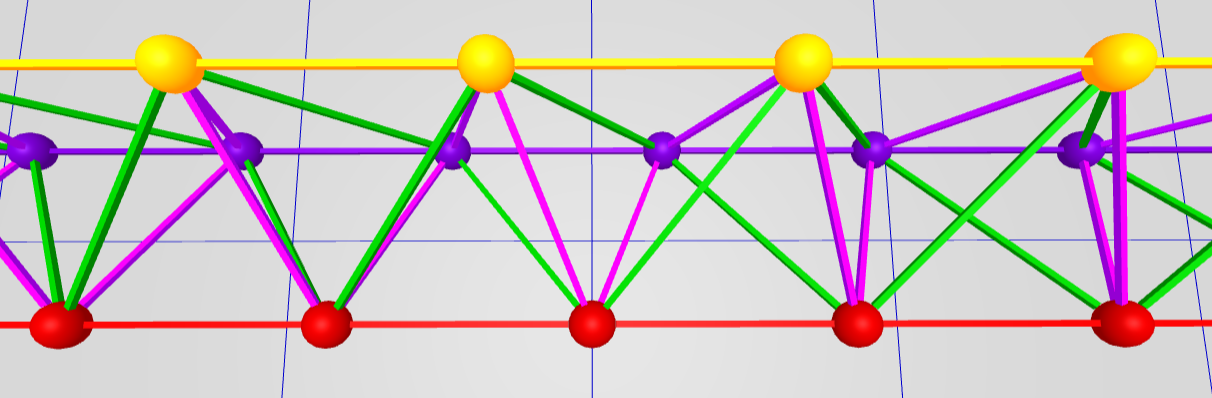
\includegraphics[width=0.65\textwidth]{figures/EquitetrabeamCloseUp.png}
     \caption{Equitetrabeam, an irregular tetrahelix}
  \label{fig:equitetrabeam}
\end{figure}

In order to investigate irregular simplex chains, a software platform for tetrahedral chains similar to the 2D website we have build would be
extremely useful.

\begin{problem}[SOFTWARE FOR REGULAR/IRREGULAR TETRAHEDRAL CHAINS]
(Hard 8) Can we create a browser-based software toolkit that allows us to with regular or irregular tetrahedral simplex chains.  
\end{problem}

\begin{itemize}
\item (Medium 6 I3D-07) What change length is required to make a finger ring?
\item (Hard 8 I3D-08) Clearly Equitetrabeams are stackable, in fact you can make a hexagon of them. Can we make a twisted tetrabeam with 3 or 6 columns that is even more efficient (in terms of the ratios of edge lengths)?
\item (Medium 7 I3D-09) What is the minimum change length to make a torus?
\item (Medium 6 I3D-10) What is the minimum change length of a tetrobot that can touch its toe?
\item (Hard 8 I3D-11) What is the densest way to pack a tetrobot into a given volume? (Bounds acceptable)
\item (Hard 8 R3D-12) Can we develop math for ``regular variations'' (no kinks)?
\item (Hard 8 R3D-13) Can we develop math for ``one kink'' regular variations?
\item (Hard 10 I3D-14) Can we make a torus that turns itself inside out via continuous changes of edge lengths,
  creating circular motion of a point around cross-section of torus? (In a sense, this would be a nano-technology motor.)\footnote{I might attack this problem by attempting to disprove it, and then writing code to make it happen if I could not disprove it/}
\item (Hard 8 I3D-15) Is there a formula for producing a helix of tetrahelices?
\item (Hard 8 I3D-16) Is there a way to ``knit'' Tetrahelices into  a slab?\footnote{This is poorly defined.}
\item (Hard 8 I3D-17)Is there a way to ``wind'' tetrahelices into column?
\item (Hard 8 I3D-03) How fast can the tip of a tetrahelix move given a rate of change of member length? Can we define a this derivative with a closed form expression, rather than using matrix-based arbitrary Jacobians?
\item 
\end{itemize}

Define {\em point reachability} to mean place the apex of a simplex chain near a point.
\begin{itemize}
\item  (Medium 7 R2D-03) In 2D, give an algorithm that produces the shortest regular simplex chain coming as close as possible to a point.
\item (Hard 7 R3D-22) Given a limit to the number of simplices, what is the reachable space to with distance $x$?
\item (Hard 9 I3D-23) What is the shape of reachable points for $N$ simplices?
  \item (Hard 9 I3D-24) In 3D, given an algorithm that produces the shortest simplex chain that comes with $x$ of a target point.
  \end{itemize}



\section{Hunting techniques}

In hunting for these open problems, it would be nice to define a toolkit of techniques that we can use.

The 2D website that we have made for testing 2d-regular generators is a valuable tool.
It would be nice to have such a website that supports irregular triangles as well.

Although more challenging, we could also produce software to test 3D simplex chains.
If someone would do this as early in the Mathathon as possible, this would obviouosly be extremely valuable.

The author is familiar with computer science techniques. Mentioning mathematical techniques useful in addressing these problems would be
very appreciated.

\section{G-Brain's relation to other mathematics}

In comments in a Reddit post, \url{https://www.reddit.com/r/math/comments/9l4qmw/a_mathathon_a_cooperative_free_virtual_hackathon/},
G-Brain point out this a simplex chain can be related to typical mathematical language:
\begin{quote}
  I would say a simplex chain is a (countable) pure simplicial $d$-complex in $R^d$ such that its facet graph (vertices are facets, edges are between facets which meet in a codimension 1 face) admits a Hamiltonian path (visits each vertex exactly once, without repetition of vertices or edges).
\end{quote}
We have not emphasized this language because it seems more user-friendly to approach some of the problems from the position of Computer Science than from pure mathematics.

\section{Rules of the Mathathon}

\subsection{Rules}

The intention of the Mathathon is to perform all the work in the light and to encourage math
as a social activity.
It is our hope that all members will add their written work to a GitHub repo as quickly
as they can---for example, every 30 minutes or more often would not be unreasonable.
To be eligible for an award on the basis of content, all content must be published in a GitHub repo
whose entire contents are licensed under Create Commons By Attribution(0), or the
participant must permit their work to be so published in writing.
These repos must remain publicly accessible for one month after the date of the hackathon.

It is preferable to name one file in each repo ``FinalSubmission.pdf'', with the expectation that this
will be the first file read by the judges, and that this file may be included in proceedings, if the
organizers choose to create a proceedings publication.

However, to be considered for an
award all material must be placed in public GitHub repo, or emailed in a pdf before a deadline.
The deadline for email submissions may be early than the deadline for GitHub repo-based submissions.

\subsection{Awards}

Awards at present do not have monetary prizes. If a sponsor provides monetary support, my current intention is to split
the award money evenly between each category below. Participants may receive more than one award.

If sufficient people volunteer, judging will be by a panel of judges.

Awards will be given for:
\begin{itemize}
\item Crowd favorite (to be determined by email vote)
\item Best contribution by someone without a post-baccalaureate degree
\item Best contribution by someone without a college degree
\item Best contribution by someone without a High School degree
\item Best contribution by a Senior Citizen (at least the age of 65)
\item Most creative technique
\item Best contribution by someone not a US Citizen
\item Most worthy of publication
\item Second most worthy of publication
\item Best contribution by a child under 16 (may be accomplished in conjunction with a coach, so long as the child is fully engaged)
\item Best contribution of a new problem statements
\item Most helpful to other participants (not on same team), to be awarded based on written testimonials
\item Second most helpful to other participants (not on same team), to be awarded based on written testimonials
\item Most useful open repo during the mathathon
\item Best mathematical presentation and writing
\item Best code contribution
\item Best contribution of graphic art, figure, or diagram
\end{itemize}

\section{Key Personnel}

Robert L. Read, PhD

\subsection{Potential Key Personnel}

\begin{itemize}
\item David Jeschke
  \item Stephanie Liu
\end{itemize}


\bibliographystyle{unsrt}
\bibliography{gluss}

\section{Acknowledgement}

Many thanks to David Jeschke for assisting in writing the test software.

Thanks to G-Brain of Reddit for relating this to typical mathematical language.

Thanks to Stephanie Liu for promotional assistance.

\appendix{Is there a rule that produces ``straight'' 4D simplex chains?}

If we imagine moving into a four dimensional space, does it make sense to imagine a simplex chain, even though this will have
not solid physical reality as we know it.

The ``face'' of such a figure is in face a 3-dimensional shape, can ``adjoining'' means that two 4D simplices have faces in the same 3D volume.

Possibly we could write a computer program that would allow us to render projections of such figures.
I cannot imagine such shapes, and in a way they become less interesting and less practical than 3D simplex chains.
However, one question seems interesting:

Is there a rule that produces a simplex chain in 4D which would produce a ``straight'' figure?
That is, a figure which always remained within in a fixed distance of a line embedded in 4-space?

Idea: The problem doesn't limit the computational complexity of the chain rule producing the simplex.
However, if we evaluate the simplest rules first, we could write a computer program to simply try a large number
of them. A ``simple'' rule could be considered a function only of the number ``n'' modulo some small number ``m''.

If you consider only simple rules, how does a 4D simplex chain behave? Does it spiral out of control, or remain within
a finite region of space? 


\end{document}




\url{https://en.wikipedia.org/wiki/Open_problem}
